\documentclass[a4paper, 11pt]{article}
\usepackage[utf8]{inputenc}
\usepackage[T1]{fontenc}
\usepackage{polski}
\usepackage{times}
\usepackage[margin=2.5cm]{geometry}
\usepackage{wrapfig} 
\usepackage{xcolor}
\usepackage{amsmath}
\usepackage{graphicx}
\usepackage{mathtools}
\usepackage{titlesec}
\titleformat{\subparagraph}
    {\normalfont\normalsize\bfseries}{\thesubparagraph}{1em}{}
\titlespacing*{\subparagraph}{\parindent}{3.25ex plus 1ex minus .2ex}{.75ex plus .1ex}

\title{Latex - Referat}
\author{Cezary Krysztoszek}
\begin{document}
\maketitle 
\tableofcontents % spis tresci
\section{Rozdzial numerowany}
\subparagraph{Podpunkt numerowany}

\section*{Rozdzial nienumerowany}
\subparagraph*{Podpunkt}
\section {Numerowanie}
\begin{enumerate}
\item Pierwszy
\item Kolory \newline
{\color{red} Troche czerwonego} \newline % zalamanie lini
\emph{Tekst na czarno {\color{blue} Troche niebieskiego} i na koniec znowu czanry}
\end{enumerate}
\section{Tabela}
\begin{tabular}{|r|l r|}  % okresla jakiej szerokosci bedzie tabela oraz ich format r-right(prawo stronne, l-left(lewo stronny), c - centrum. Pionowe kreski reprezentują linie między tabelami
  \hline 
  pozycja 11 & pozycja 12 & pozcja 13\\
  \hline
  pozycja 21 & pozycja 22 & pozycja 23 \\
  \hline % reprezentuje dolną linie
  pozycja 31 & pozycja 32 
  
\end{tabular} 
\section{Obrazki}
\begin{wrapfigure}{r}{0.5\textwidth}
\begin{center}
\vspace{-20pt} %% odległość od górnego marginesu
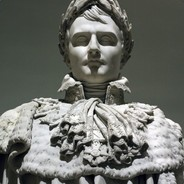
\includegraphics[width=0.48\textwidth]{obrazek1}
\end{center}
\caption{Napoleon Bonapharte}
\end{wrapfigure}
Napoleon I (ur. 15 sierpnia 1769 w Ajaccio na Korsyce, zm. 5 maja 1821 w Longwood na Wyspie Św. Heleny) – francuski wojskowy, Pierwszy Konsul Republiki Francuskiej 1799–1804, cesarz Francuzów w latach 1804–1814 i 1815, prezydent (1802–1805), a następnie król Włoch (1805–1814), Suweren Wyspy Elba (11 kwietnia 1814 – 20 marca 1815)





\newpage % kolejna strona
\section{Matematyka}
\subparagraph{Alfabet grecki, funkcje trygonmetryczne}
\begin{math}
\alpha, \beta,  \gamma
\cos (\alpha), \sin (45^\circ ), \tan\alpha
\end{math}
\subparagraph{Potęgi i Pierwiastki, i Index Dolny}
$$ C_i^2 $$
$$ \sqrt{25} = 5 $$
$$ k_0 + k_1 + ... + k_{n+1} $$ % przy dłuższych(większych niż 1 symbool) indexach dolnych i górnych należy używać nawiasów klamrowych.


\subparagraph{Ułamki}
$ \frac{25}{5} = 5 $ \newline
$ \frac{\frac{3}{6}}{123} $
\subparagraph{Operacje na zbiorach}
\begin{tabular}{| r | r |}
\hline
Symbol & Kod \\
\hline
$ \subset $ & subset \\
\hline
$ \subseteq $ & subseteq \\
\hline
$ \supset $ & supset \\
\hline
$ \supseteq $ & supseteq \\
\hline 
$ \times $ & times \\
\hline
\end{tabular}
\subparagraph{Logika}
\begin{tabular}{|r|r|}
\hline
Symbol & Kod \\
\hline
$ \neg $ & neg \\ % negacja
\hline
$ \implies $ & implies \\ % implikacja
\hline
$ \iff $ & iff \\ % rownowaznosc
\hline
$ \land $ & land \\	% koniunkacja	
\hline 
$ \lor $ & lor \\ % alternatywa
\hline
\end{tabular}
\subparagraph{Macierze}
\begin{math}
\begin{bmatrix}
       \frac{3}{7} & \frac{1}{6} & \frac{1}{4} \\[0.3em]
       \frac{5}{6} & 0           & \frac{5}{6} \\[0.3em]     
       0           & \frac{5}{21} & \frac{1}{6}
     \end{bmatrix} 
           \qquad % Dzięki temu druga macierz zostala zapisana obok pierwszej a nie pod nią  
           \begin{bmatrix}
       1 & 5 & 14 \\[0.3em]
      72 & 0  & 56 \\[0.3em]     
       0 & 52 & 4
     \end{bmatrix} 
\end{math}
\newline
\subparagraph{Układy równań}
$$
y = \left\{ \begin{array}{ll}
a & \textrm{gdy $d>c$}\\
b+x & \textrm{gdy $d=c$}\\
l & \textrm{gdy $ d < c $}
\end{array} \right.
$$
$$
y = \left\{ \begin{array}{ll}
x+y^2 = 12 \\
6x+4 = 15 \\
y-x = 7
\end{array} \right.
$$
\newline
\newpage
\section{Inne różności}
\subsection{Flushleft i Flushright, i center}
\begin{flushleft}
To jest tekst\\
wyrównany do lewej.\\
\end{flushleft}
\begin{flushright}
To jest tekst\\
wyrównany do prawej.\\
\end{flushright}
\begin{center}
To jest tekst\\
wyrównany do środka.\\
\end{center}
\subparagraph{Dodatkowe znaki}
\begin{tabular}{| r | r |}
\hline
Symbol & Kod \\
\hline
$ \neq $ & neg \\
\hline
$ \geq $ & geq \\
\hline
$ \leq $ & leg \\
\hline
$ \in $ & in \\
\hline
$ \exists $ & exists \\
\hline
$ \forall $ & forall \\
\hline
\end{tabular}
\section{Zadania}
Zadania 1:\newline
Za pomocą tabeli sprawdz wartość zdania logicznego dla każdej możliwej zmiennej: \newline
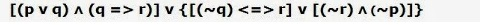
\includegraphics{zadanie1}
\newline
Zadanie 2:
Za pomocą funcji bmatrix wykonaj zadania: \newline
a) A + B\newline
b) A - B\newline
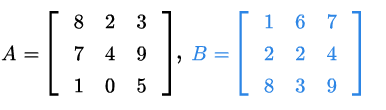
\includegraphics{zadanie2}\newline
Zadanie 3: \newline
Napisz w LaTex-ie dane równaniania matematyczne: \newline
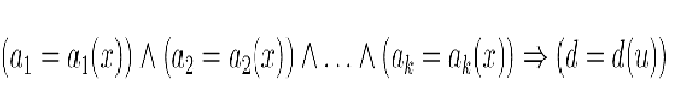
\includegraphics{zadanie3}\newline
\end{document}